\newpage
\begin{tikzpicture}[remember picture, overlay]
	\node [inner sep=0pt, minimum width=\paperwidth, minimum height=\paperheight] at (current page.center) {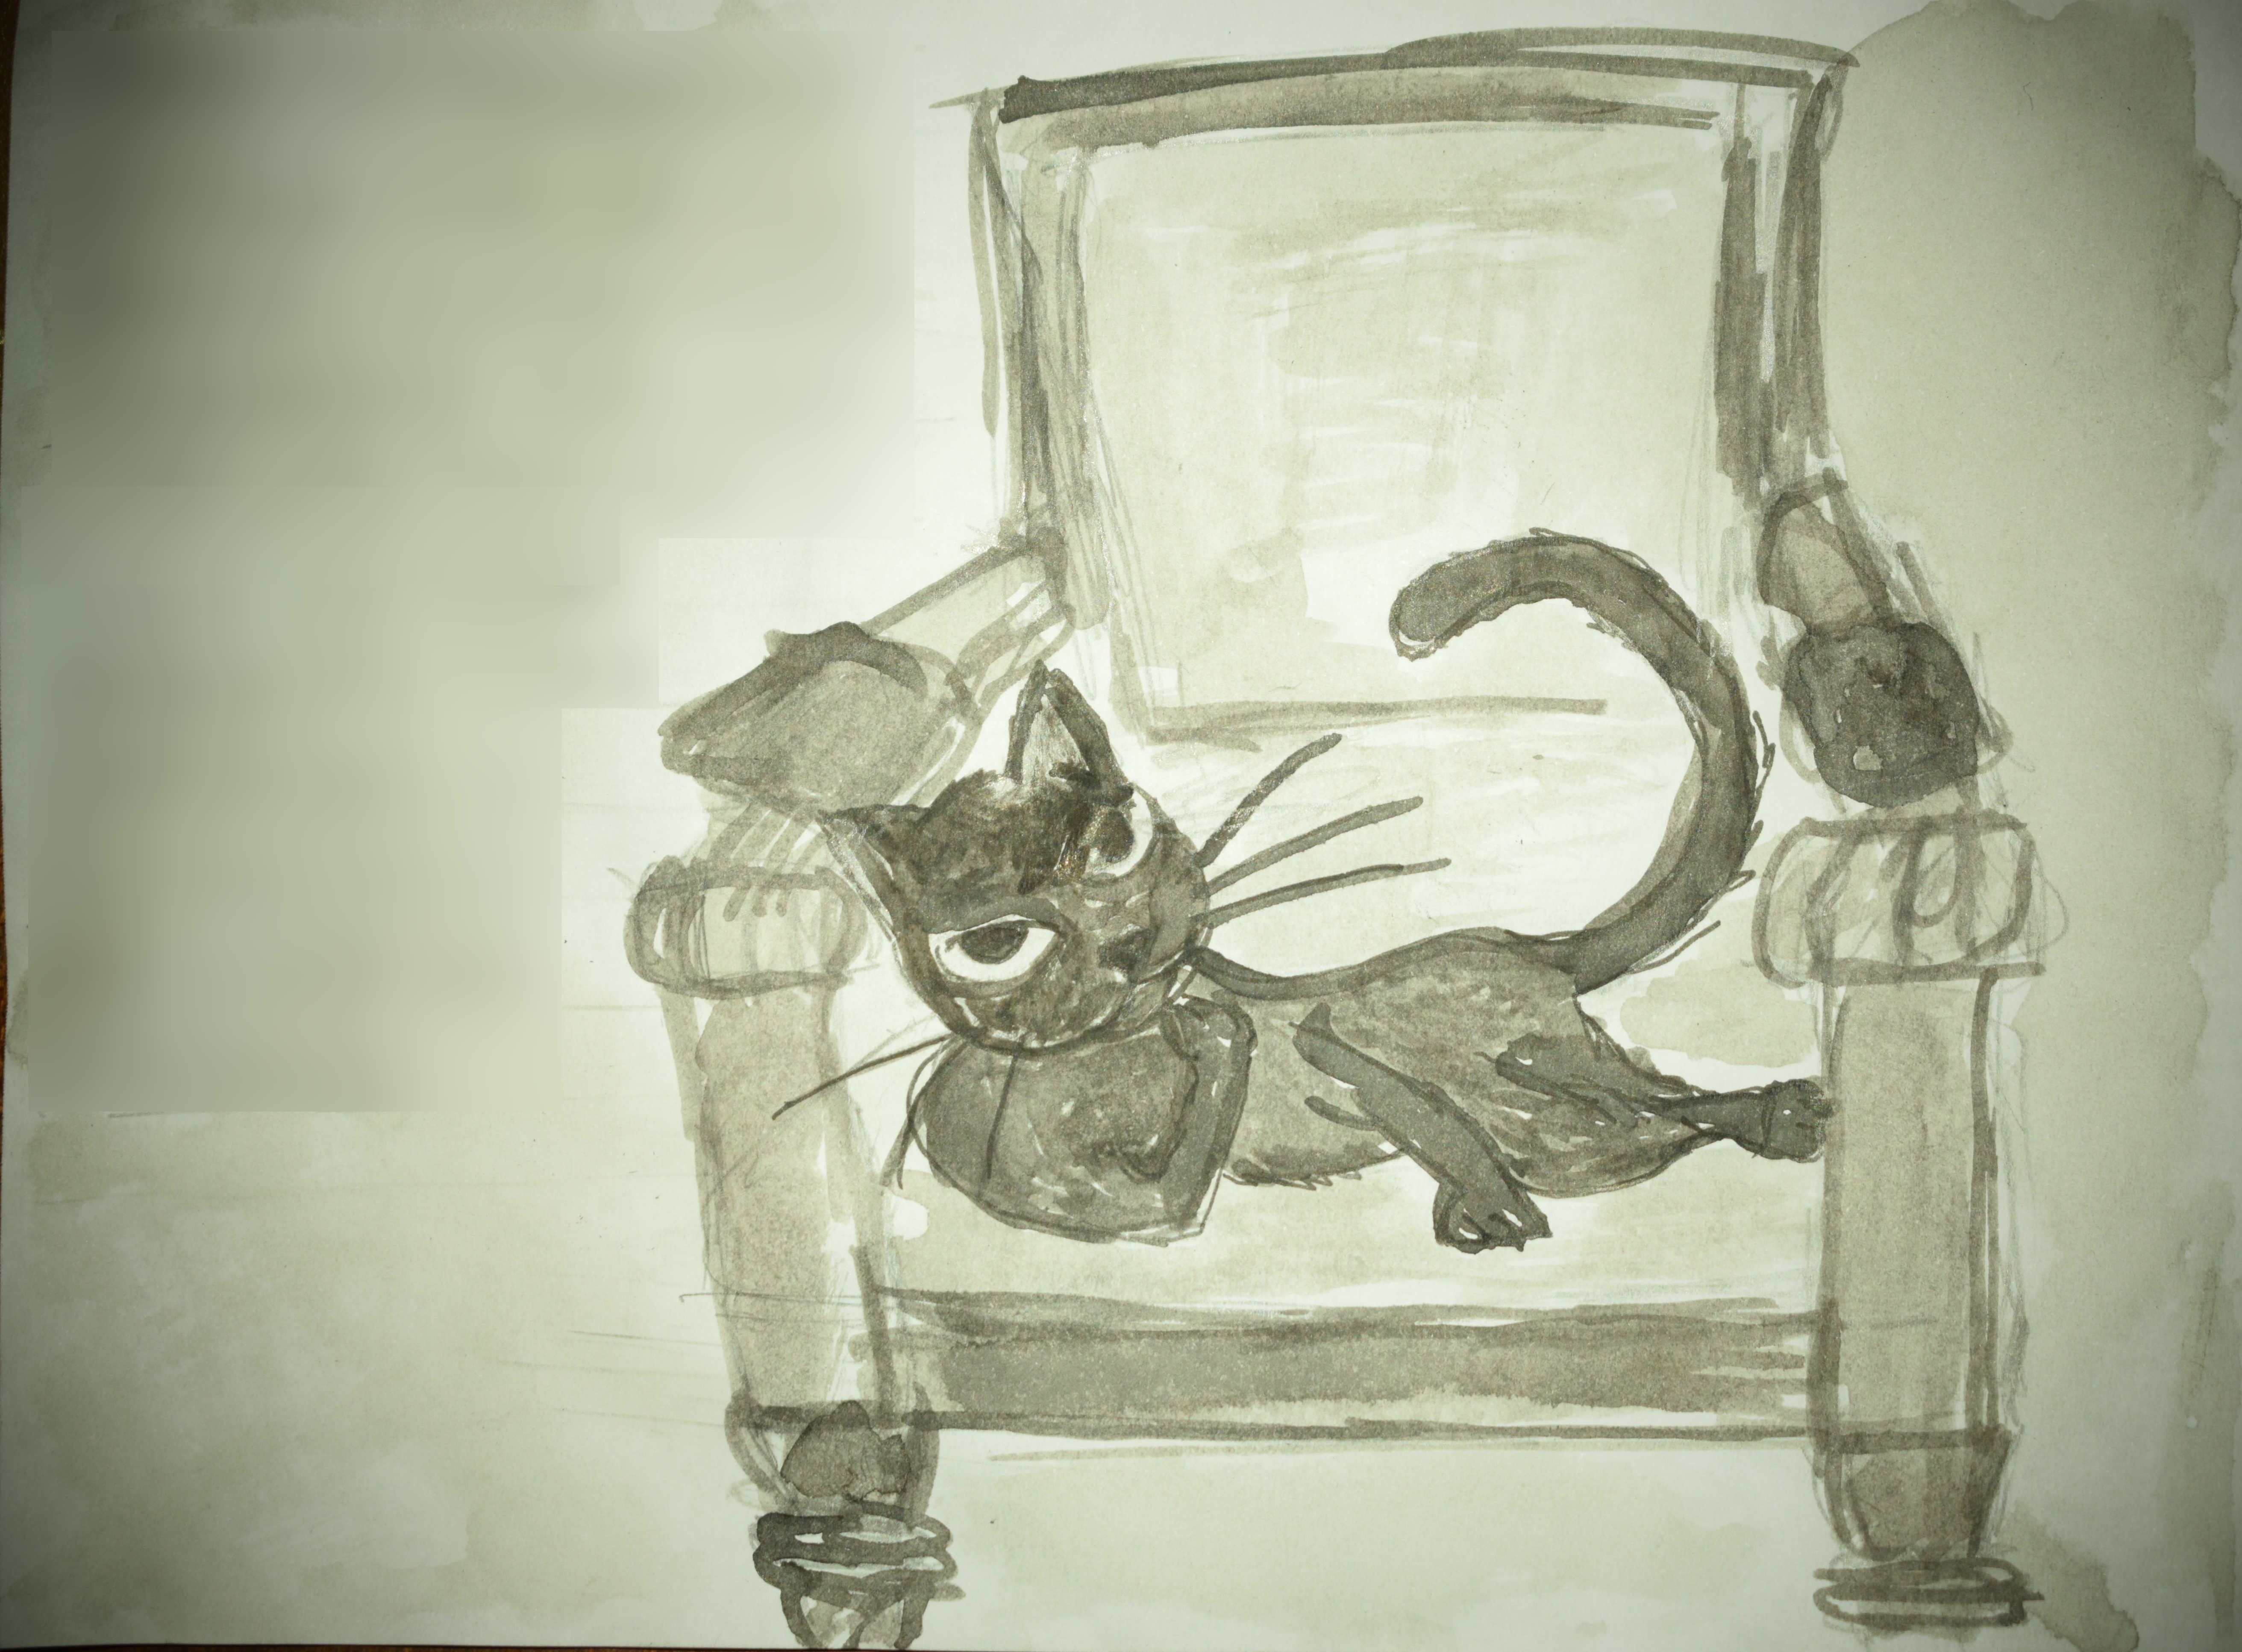
\includegraphics[width=\paperwidth,height=\paperheight,angle=0]{presenta}};
\end{tikzpicture}
%\end{normal}
%\begin{minipage}{.35\textwidth}

HOLA, MI NOMBRE ES OTTOKO, VIVO EN VILLA DEVOTO. 

SI BIEN PUEDE PARECERLES QUE LLEVO UNA VIDA 

APACIBLE Y HASTA UN TANTO PEREZOSA, 

VOY A 

CONTARLES 

LA ÚLTIMA 

DE MIS 

INTRÉPIDAS

AVENTURAS.	


%\end{minipage}	

\newpage
\begin{tikzpicture}[remember picture, overlay]
	\node [inner sep=0pt, minimum width=\paperwidth, minimum height=\paperheight] at (current page.center) {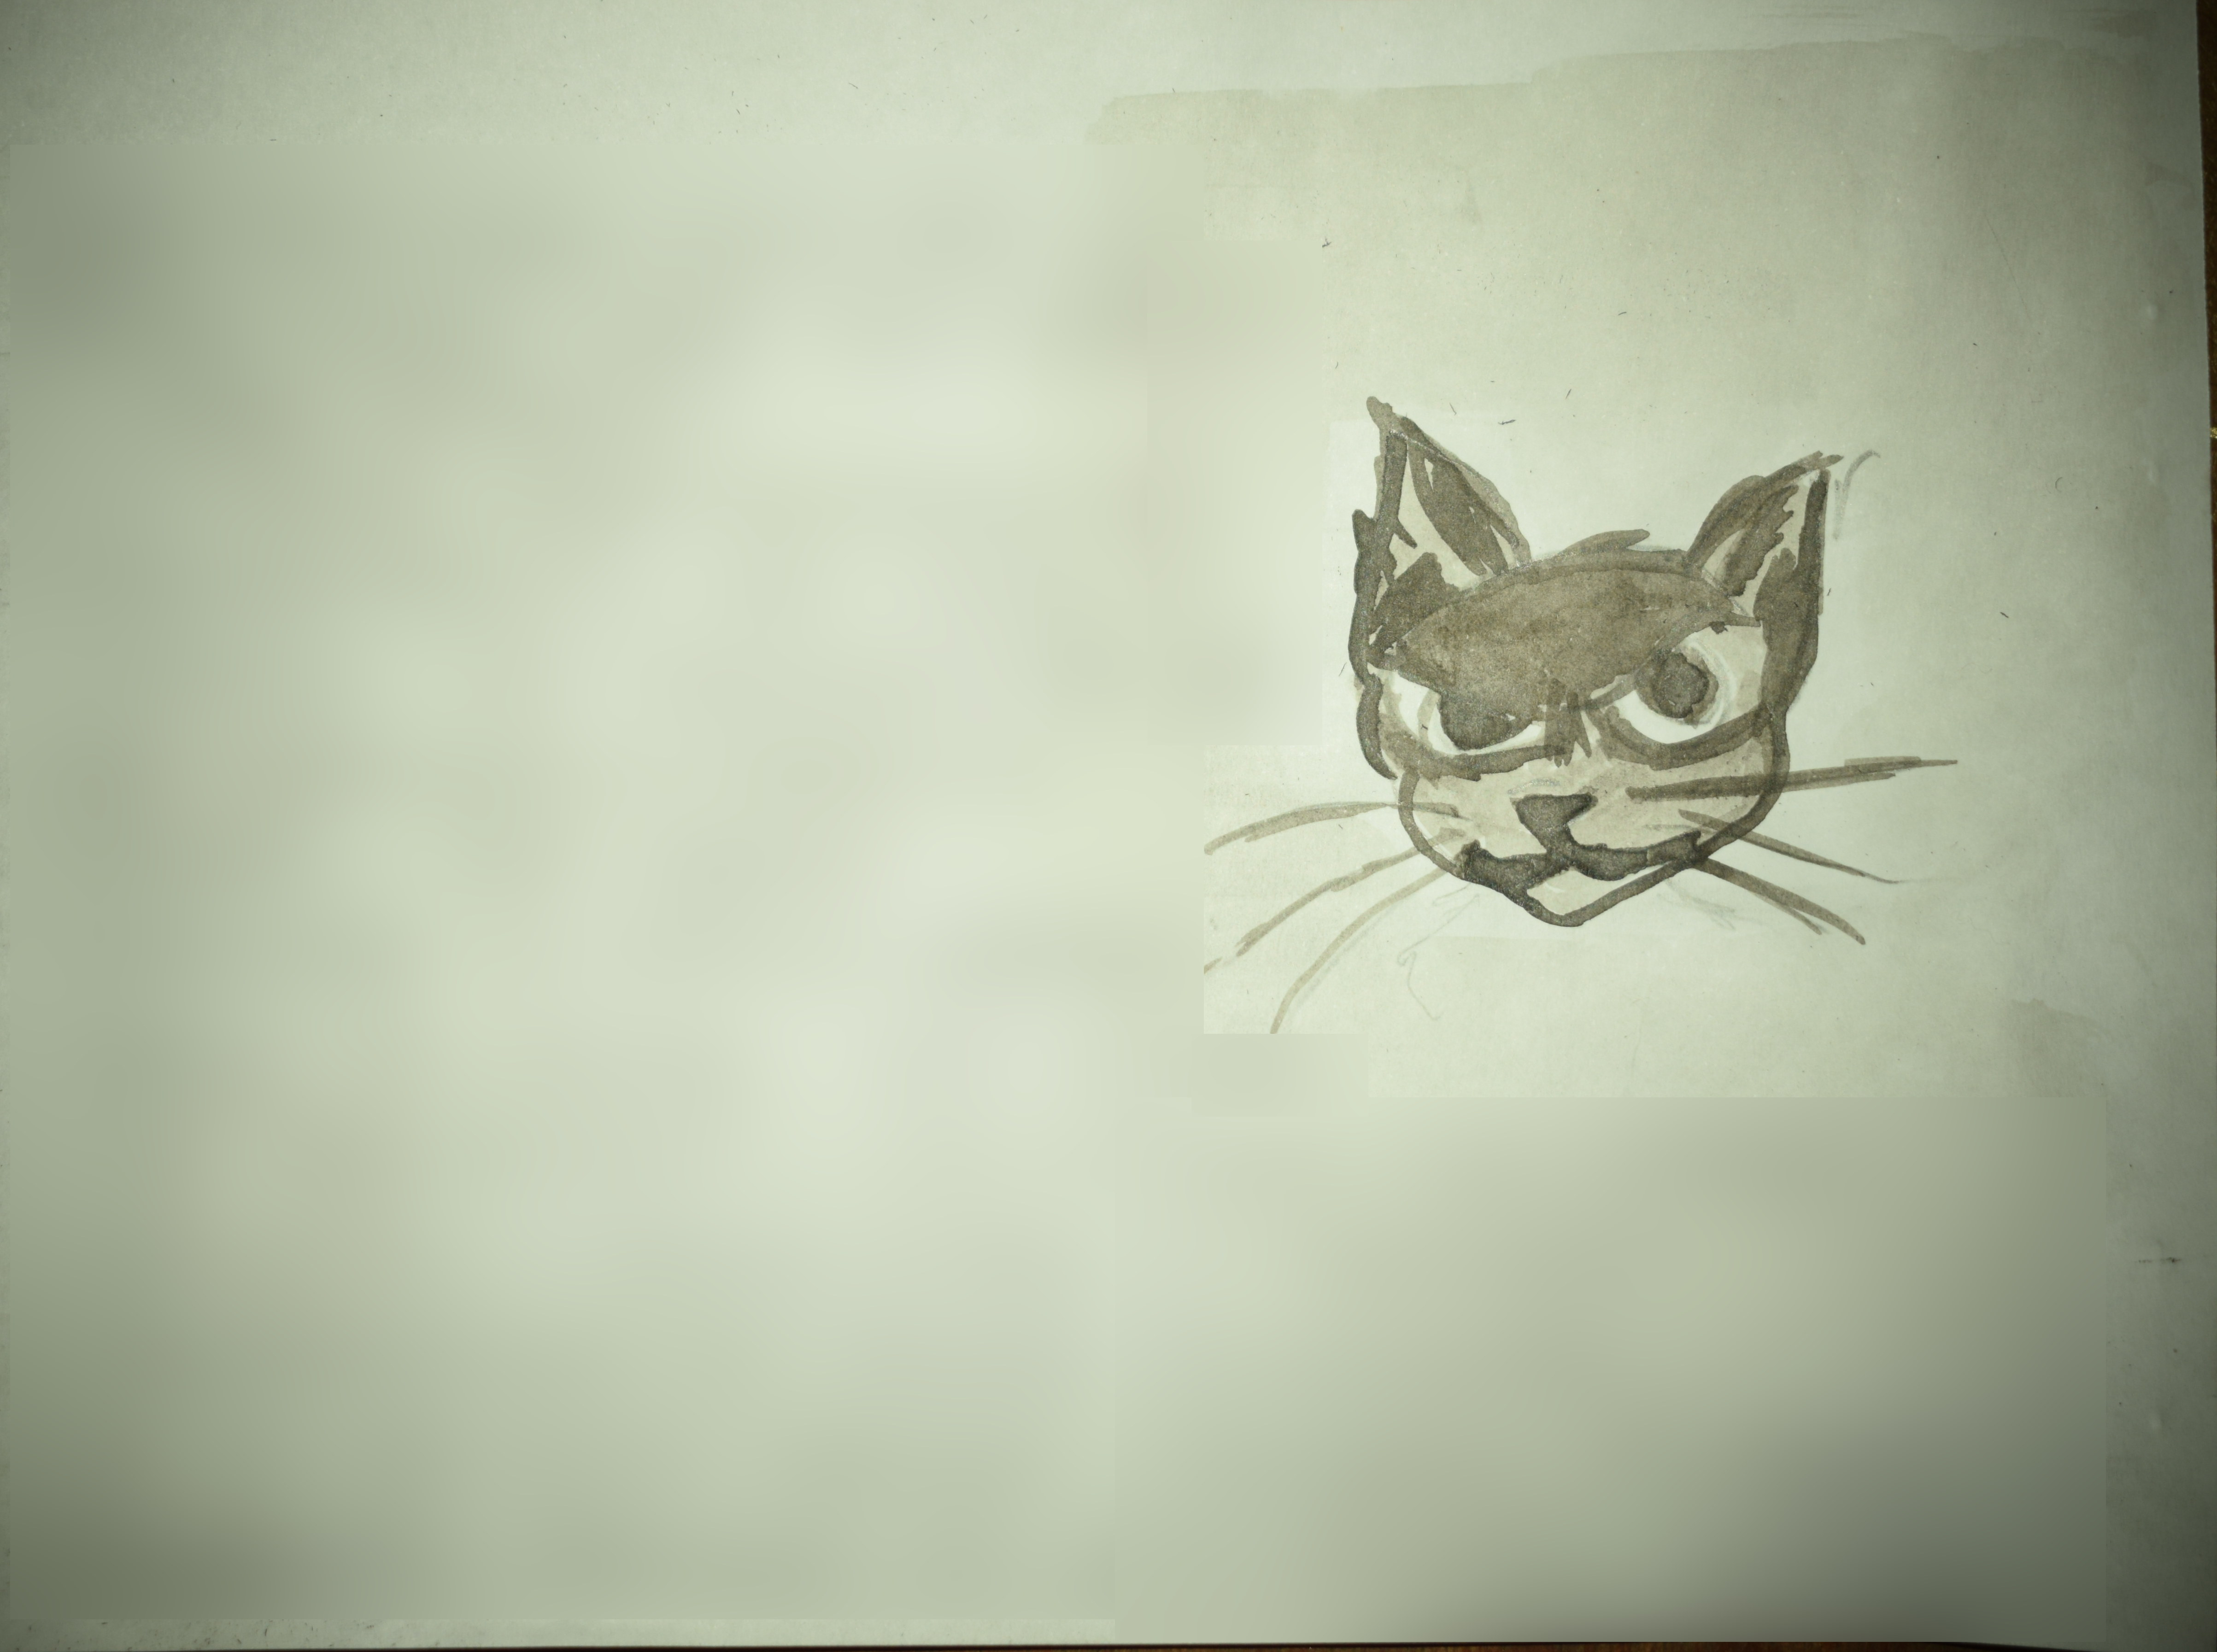
\includegraphics[width=\paperwidth,height=\paperheight,angle=0]{presenta2}};
	
	\node[text width=\textwidth,xshift=0cm,yshift=0cm] at (current page.center){PUEDE QUE ALGUIEN DESCONFÍE DE LOS RELATOS DE UN GATO NEGRO, $\ldots$ ¿QUIÉN NO HA ESCUCHADO DECIR QUE LOS GATOS NEGROS TRAEMOS MALA SUERTE? ¡PURAS PATRAÑAS! 
		
		A VECES, REPETIR COSAS SIN PENSAR 
		
		RESULTA 	
		FÁCIL Y CÓMODO. POR ESO, AÚN
		
		HOY HAY 	
		PERSONAS QUE CREEN QUE EL 
		
		PLANETA 	 
		TIERRA	 
		ES PLANO, QUE LA 
		
		ASTROLOGÍA	  
		SIRVE	  
		PARA   
		CONOCERSE,
		
		QUE EXISTEN
		EL MAL	  
		DE OJO 	  
		Y LAS BRUJERÍAS$\ldots$ LOS HUMANOS 
		
		SON CAPACES DE ÉSTAS
		
		Y TANTAS OTRAS SANDECES CUANDO NO TIENEN GANAS DE RAZONAR. 
		
	};
	
	
\end{tikzpicture}
\newpage
\begin{tikzpicture}[remember picture, overlay]
	\node [inner sep=0pt, minimum width=\paperwidth, minimum height=\paperheight] at (current page.center) {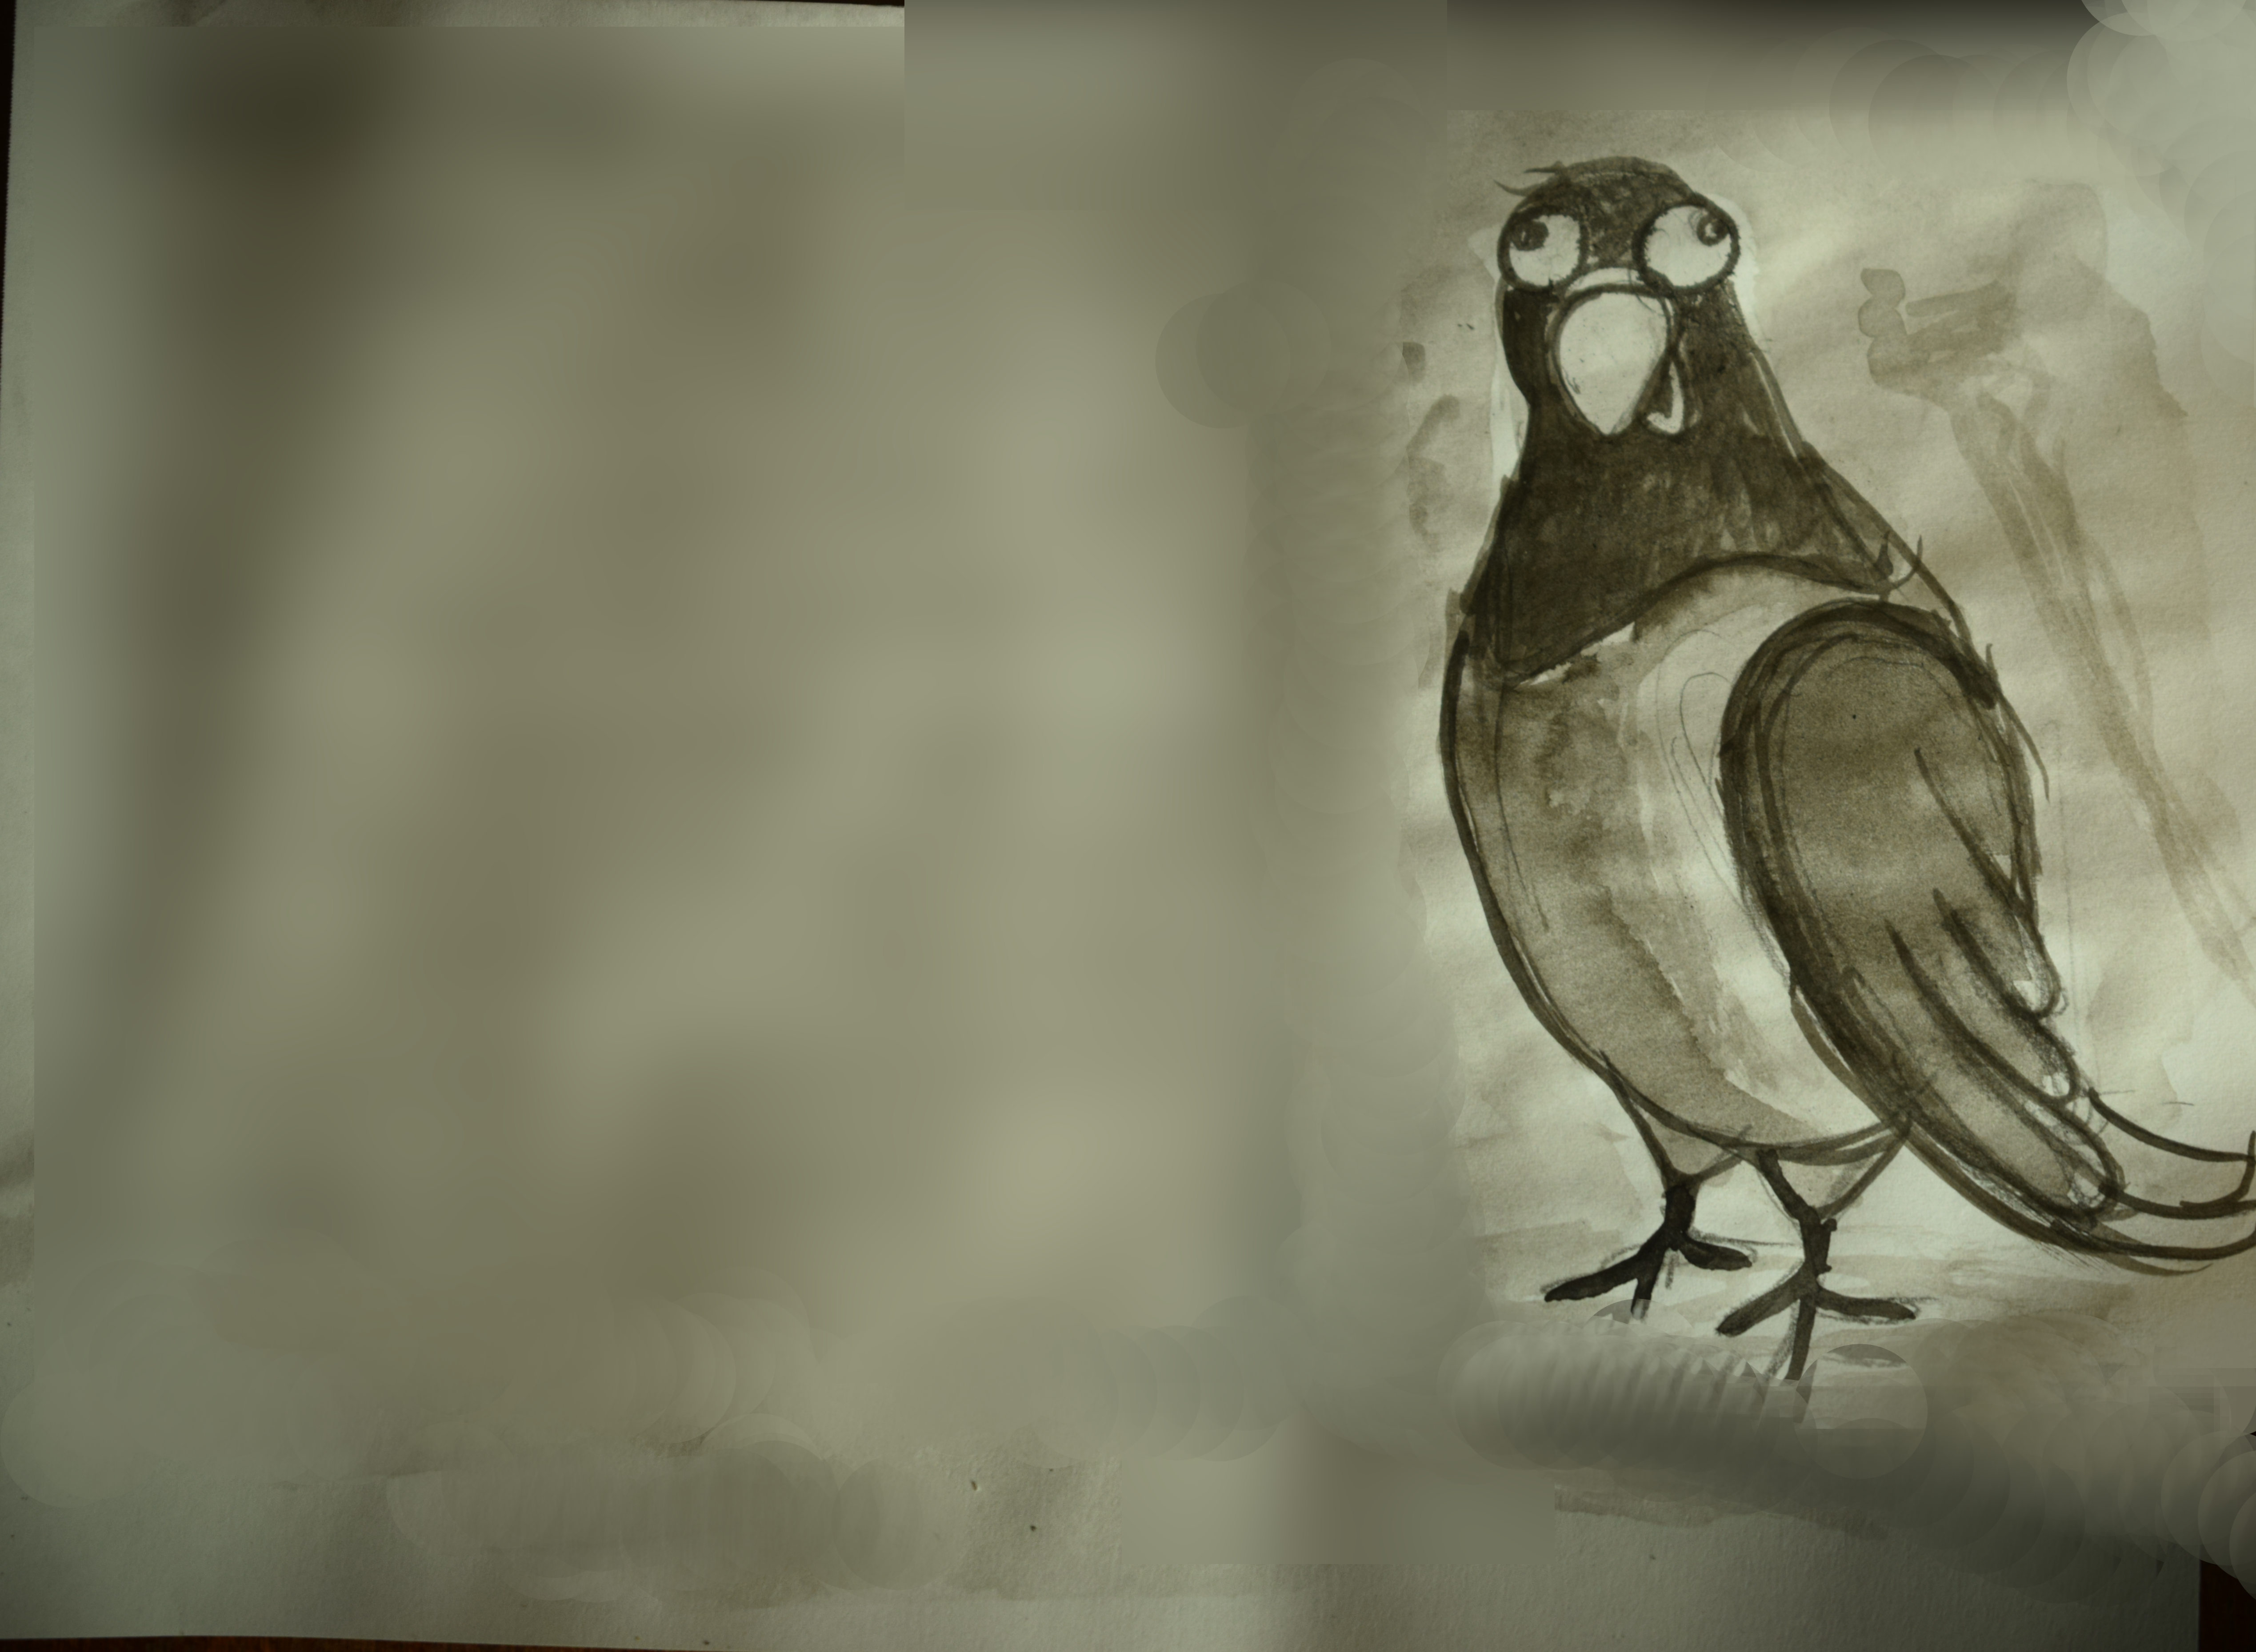
\includegraphics[width=\paperwidth,height=\paperheight,angle=0]{paloma1}};
	\node[text width=3.5cm,yshift=4.75cm,xshift=.45\textwidth] at (current page.center){¡UH! ¡UH! ¡UH!};
\end{tikzpicture}	
A MÍ ME GUSTA PENSAR.

DE OTRA FORMA SERÍA DIFÍCILMENTE UN 

BUEN CAZADOR FELINO. SEPAN QUE YA				

DESDE CHIQUITO, ME INTERESABA 

REFLEXIONAR 			 
SOBRE CÓMO ATRAPAR 

PALOMAS.

¡PALOMAS! ALGUNOS CAMARADAS LAS 
LLAMAN 			

RATAS DEL AIRE.   
¡PERO SÍ!, LOS 
GATOS 

SABEMOS QUE  			 
EXISTEN LOS			 
MURCIÉLAGOS

SIN EMBARGO, HAY MUCHOS MENOS  	DE ELLOS 

QUE  PALOMAS EN LAS CIUDADES. ESTAS AVES			

ADAPTARON SU PLUMAJE  AL COLOR 	DEL CEMENTO 

DE LOS EDIFICIOS,  DEL ASFALTO, DE LAS CALLES, 

AUNQUE, PARA MÍ, IMITAN MÁS BIEN AL TINTE DE LA MUGRE.	

\newpage
\begin{tikzpicture}[remember picture, overlay]
	\node [inner sep=0pt, minimum width=\paperwidth, minimum height=\paperheight] at (current page.center) {\includegraphics[width=\paperwidth,height=\paperheight,angle=0]{paloma2}};
\end{tikzpicture}
SI BIEN DE MIRADA TORPE 

Y DE CAMINAR MUY POCO ELEGANTE, 
\newline\newline\newline

RECONOZCO QUE SON MUY ASTUTAS

PARA EMPRENDER EL VUELO.
\newline\newline
\begin{flushright}
	\begin{minipage}[r]{.5\textwidth}
		TAMBIÉN ADMIRO ALGUNA DE SUS HABILIDADES MUY PRÁCTICAS PARA LA VIDA COTIDIANA, ¡ Y SIN PIEDRITAS!
	\end{minipage}
\end{flushright}	







\newpage
\begin{tikzpicture}[remember picture, overlay]
	\node [inner sep=0pt, minimum width=\paperwidth, minimum height=\paperheight,opacity=0.9] at (current page.center) {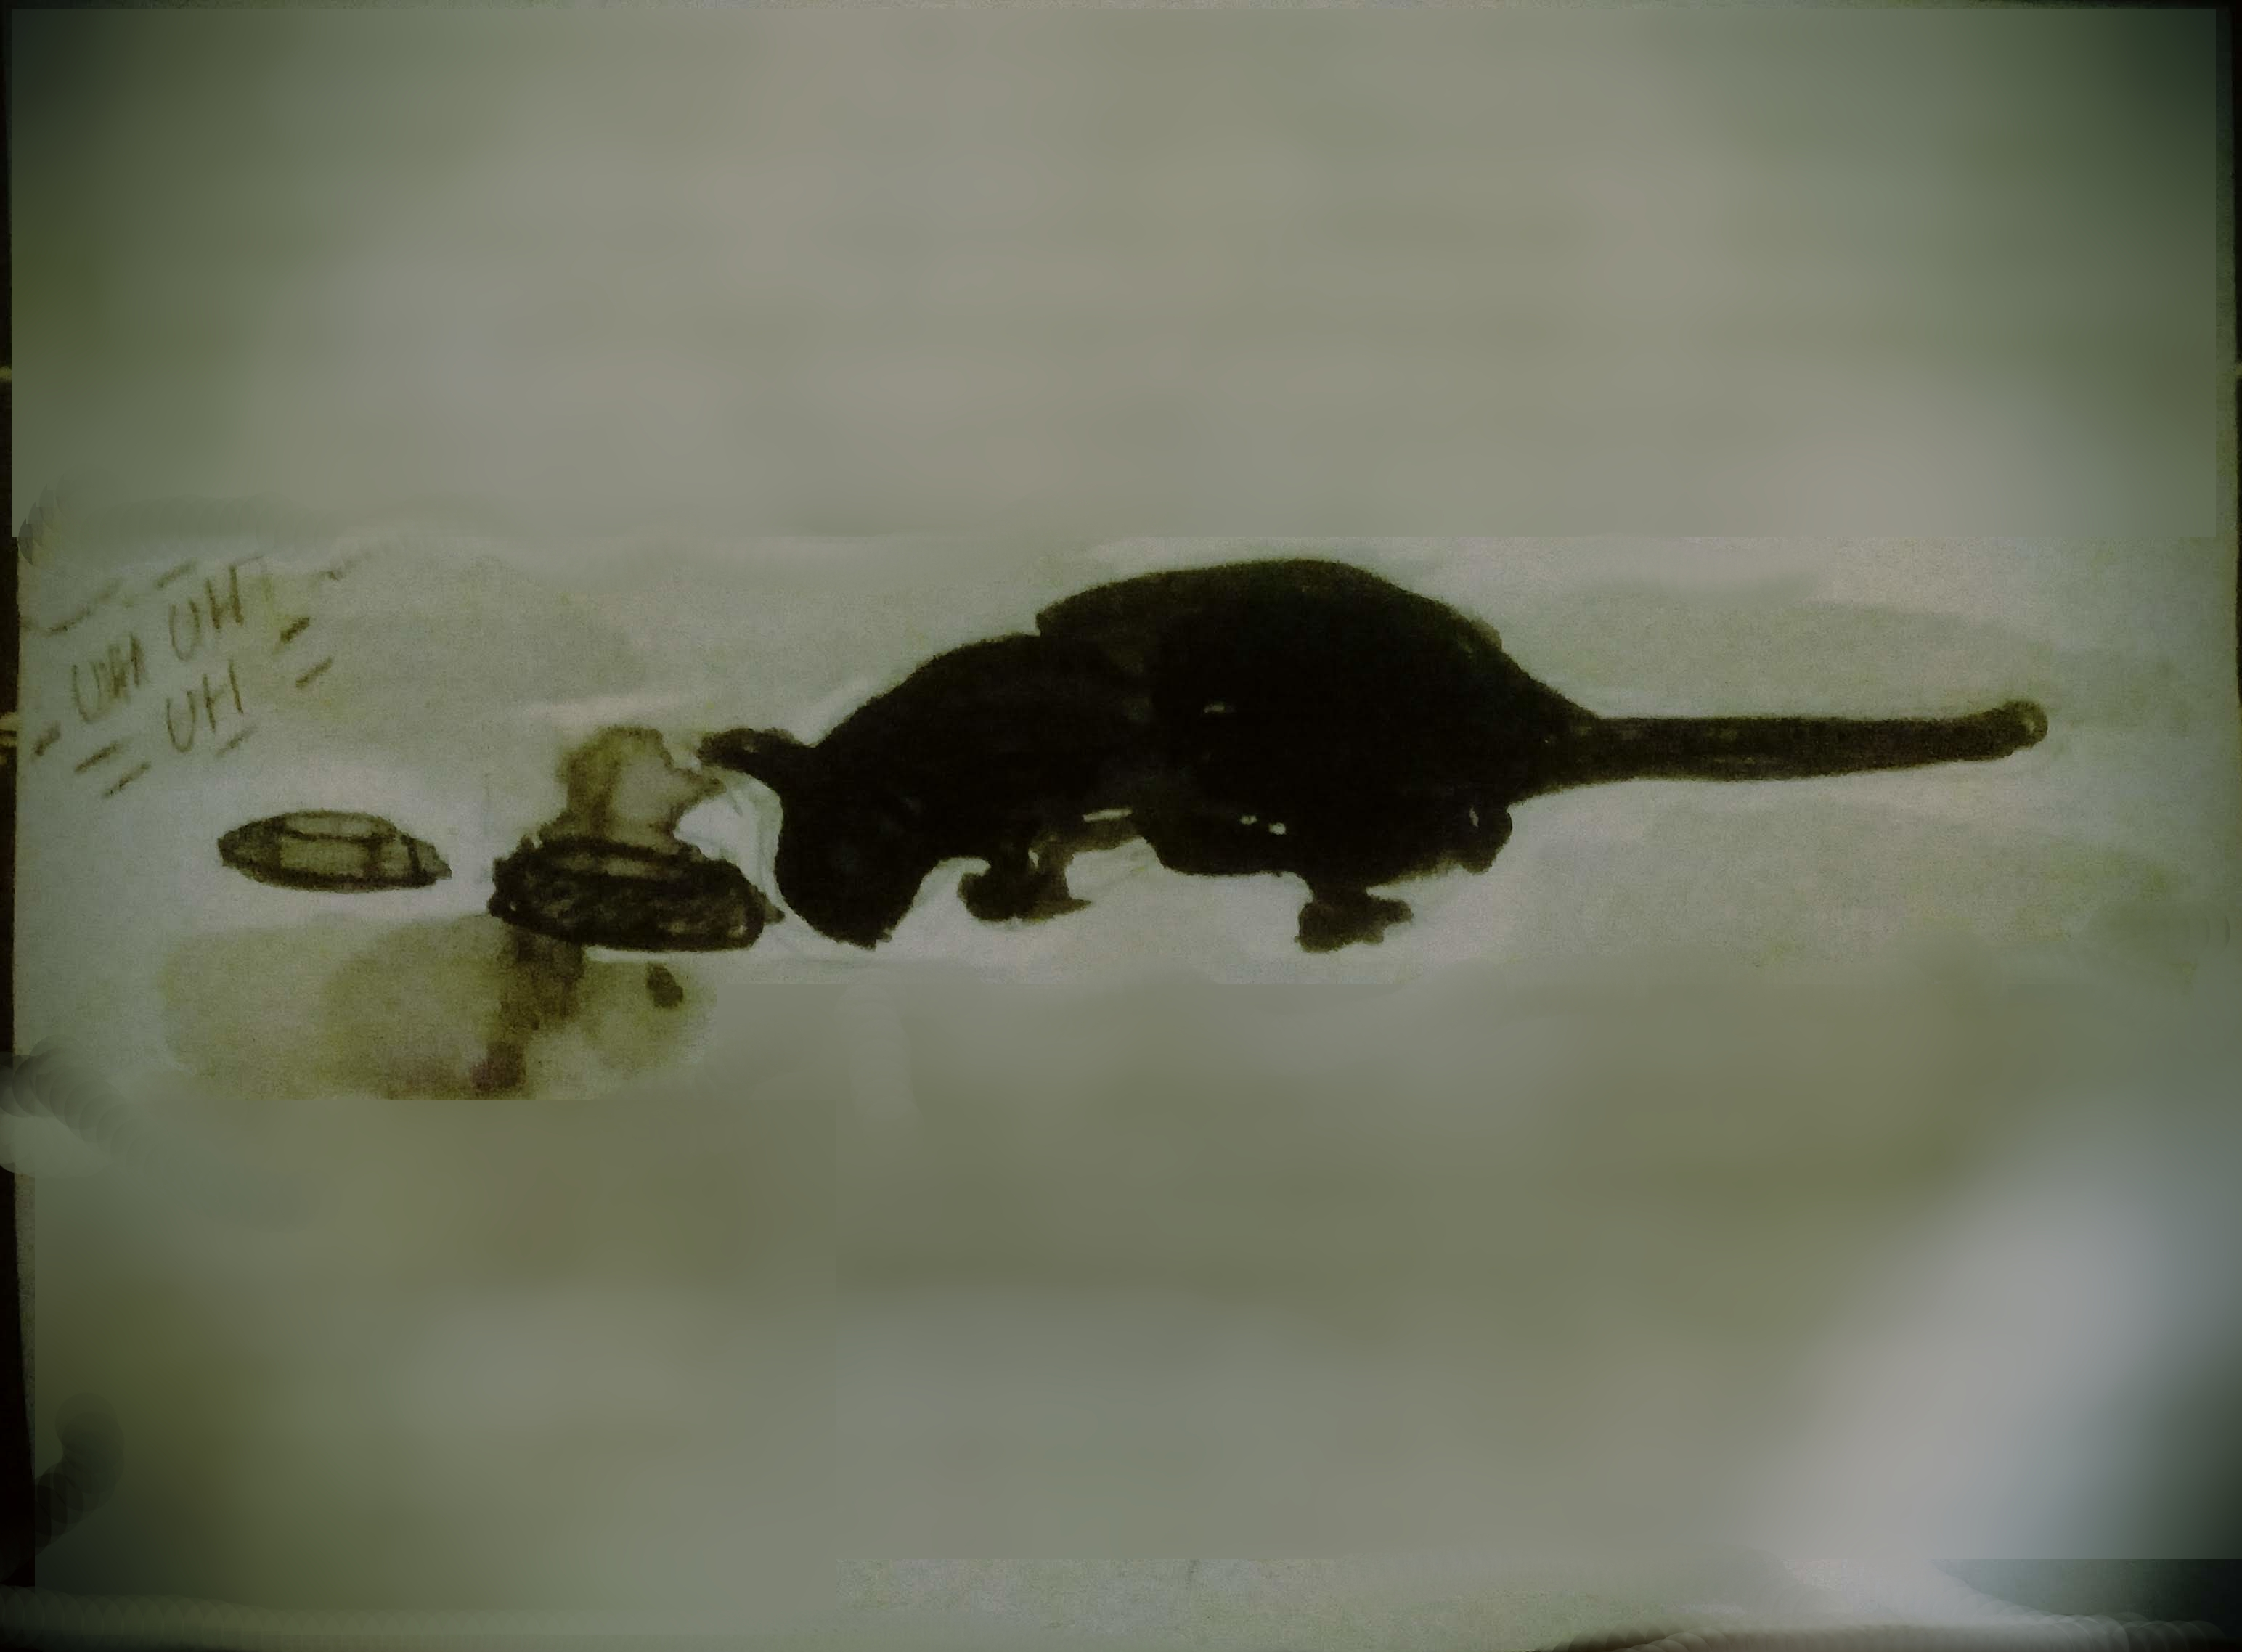
\includegraphics[width=\paperwidth,height=\paperheight,angle=0]{comiendo}};
\end{tikzpicture}	
PUES ME ENCONTRABA MUY TRANQUILO UNA MAÑANA COMIENDO MIS DELICIOSAS CROQUETAS PARA GATO (A VECES CONFIESO QUE ME HE DESAYUNADO CUCARACHAS PERO ESA ES OTRA HISTORIA) 
\newline\newline\newline
\newline\newline\newline	\newline\newline 
CUANDO ESCUCHÉ DESDE EL PATIO EL ARRULLO DE UNAS PALOMAS.
ESTABA ABIERTO EL VENTANAL Y DECIDÍ DAR UN VISTAZO . ALLÍ ESTABAN, CHARLANDO ENTRE ELLAS. CON MI HABITUAL CURIOSIDAD FELINA, ME ACERQUÉ UN POCO HACIA DONDE ESTABAN.






\newpage
\begin{tikzpicture}[remember picture, overlay]
	\node [inner sep=0pt, minimum width=\paperwidth, minimum height=\paperheight] at (current page.center) {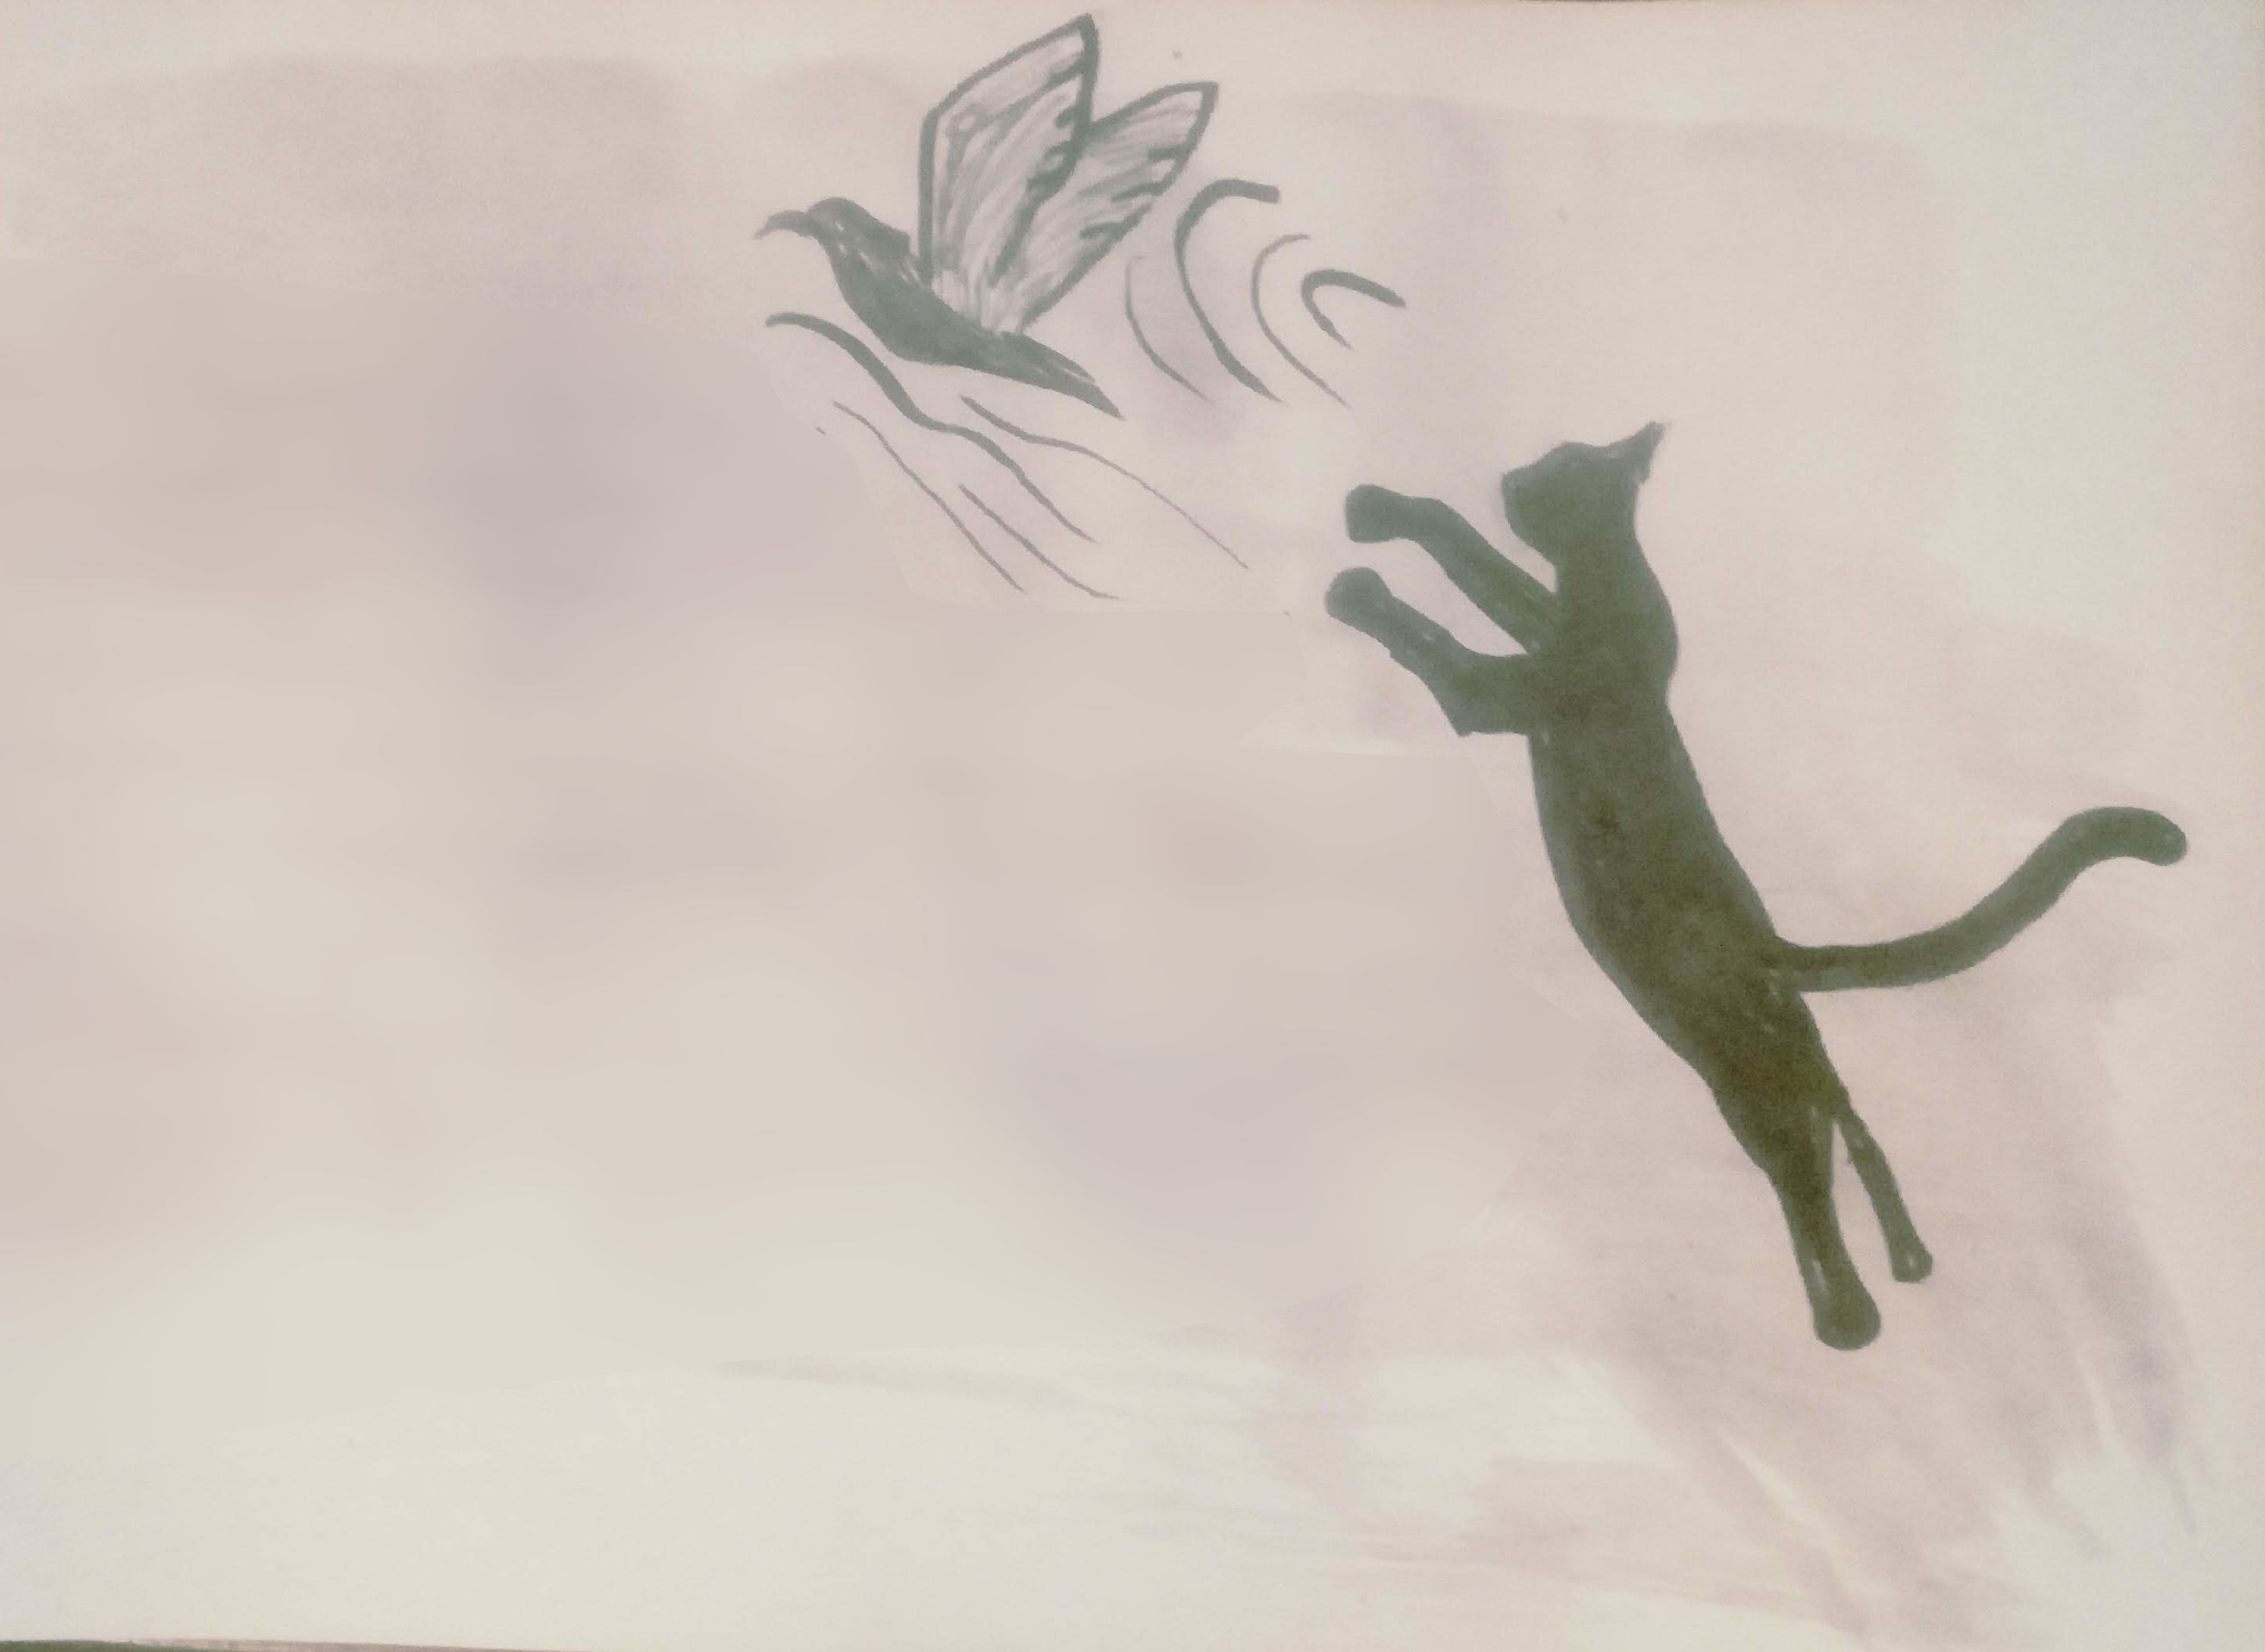
\includegraphics[width=\paperwidth,height=\paperheight,angle=0]{salto_paloma}};
\end{tikzpicture}	
CASI AL INSTANTE \hspace{.3\textwidth}¡VI QUE ME HABÍAN ENGAÑADO! 

PUES UNA AVE \hspace{.3\textwidth}INSOLENTE, HABÍA APROVECHADO 

MI DISTRACCIÓN 

PARA SAQUEAR 				
MI PLATO.

REACCIONÉ.

SI BIEN FUE UNO			
DE MIS MEJORES		

SALTOS, NO CONSEGUÍ 			  
ATRAPARLA. ¡UN GATO 

JOVEN COMO YO TENDRÍA MÁS

OPORTUNIDADES EN EL FUTURO! 

DESDE LO ALTO DEL MURO, LAS 			  
PALOMAS SE

BURLABAN DESCARADAMENTE. 

SÍ, O AL MENOS ESO PENSÉ DE LOS MÚLTIPLES 

'UH-UH-UH' QUE LLEGABAN A MIS OÍDOS.

ALGO FURIOSO, DECIDÍ DARLES UNA LECCIÓN DE HUMILDAD.


